\noindent\textbf{1.1} Phương trình trạng thái khí lý tưởng:
\begin{equation*}
  PV = \nu RT \implies R = \frac{PV}{\nu T} = 8{,}31~\text{Pa} \cdot \text{m}^3 / (\text{mol} \cdot \text{K})
\end{equation*}
Thay các đơn vị đo tương ứng, ta được giá trị của hằng số khí lý tưởng trong hệ GLA:
\begin{equation*}
  R = 8{,}23 \times 10^{-2}~\text{atm} \cdot \text{l}/(\text{mol} \cdot \text{K})
\end{equation*}

\noindent\textbf{1.2} Ở nhiệt độ $t_0 = 0^\circ$C và áp suất $P = 1{,}00~\text{atm}$, 1 lít nước hoà tan được $k_v = 1{,}71$ lít thể tích $\text{CO}_2$. Khối lượng của khí này theo phương trình trạng thái Mendeleev-Clapeyron:
\begin{equation*}
  PV = \frac{m}{M}RT \implies m = \frac{MPV}{RT} = 3{,}35~g
\end{equation*}
Vậy hằng số Henry ở nhiệt độ $0^\circ$C là:
\begin{equation*}
  k_m = 3{,}35~g / (\ell \cdot \text{atm})
\end{equation*}
Khối lượng khí hoà tan theo định luật Henry:
\begin{equation*}
  m = k_m PV = 20~\text{g}
\end{equation*}

\noindent\textbf{2.1} Theo định luật Dalton, tổng áp suất bằng tổng các áp suất riêng phần. Áp suất trong chai bằng tổng áp suất của hỗn hợp khí (không khí và khí $\text{CO}_2$ sinh ra). Vì thể tích phần chứa khí trong chai không đổi, áp suất không khí tỉ lệ thuận với nhiệt độ:
\begin{equation*}
  \frac{P_e}{T} = \frac{P_0}{T_0} \implies P_e = \left( \frac{T}{T_0} \right) P_0
\end{equation*}
Khối lượng khí $\text{CO}_2$ trong chai phụ thuộc vào nhiệt độ và được tính bởi:
\begin{equation*}
  m = m_0 - k_m P V_0
\end{equation*}
Áp dụng phương trình khí lý tưởng:
\begin{equation*}
  PV             = \frac{m}{M}RT = \frac{m_0 - k_m P V_0}{M} RT
\end{equation*}
\begin{equation*}
  \implies P  = \frac{m_0 - k_m P V_0}{M V} RT = \frac{m_0 RT}{M V} \left( 1 - \frac{k_m V_0}{m_0} P \right)  = \tilde{P} \left( 1 - \frac{k_m}{C_0} P \right)
\end{equation*}
Trong đó:
\begin{equation*}
  \frac{m_0 RT}{M V} = \tilde{P} = \tilde{P}_0 \cdot \frac{T}{T_0},
  \quad C_0 = \frac{m_0}{V_0}
\end{equation*}
Từ đó suy ra biểu thức cho áp suất riêng phần của $\text{CO}_2$:
\begin{equation*}
  P = \frac{\tilde{P}}{1 + \dfrac{k_m(t)}{C_0} \tilde{P}}
\end{equation*}
Đồ thị biểu diễn sự phụ thuộc của áp suất trong chai vào nhiệt độ:
\begin{figure}[H]
  \centering
  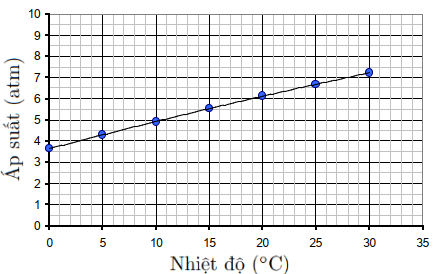
\includegraphics[width=0.5\textwidth]{Figures/Solutions/Fig 3.1.png}
\end{figure}


\noindent\textbf{2.2} Khối lượng khí hoà tan còn lại sau khi mở chai:
\begin{equation*}
  m_1 = \frac{k_0}{1 + \alpha t} P_0 V_0 = 1{,}07~\text{g}
\end{equation*}
Vậy khối lượng khí $\text{CO}_2$ thoát ra là:
\begin{equation*}
  m = m_0 - m_1 = 6{,}43~\text{g}
\end{equation*}
Thể tích khí này được tính theo phương trình trạng thái khí lý:
\begin{equation*}
  V_1 = \frac{mRT}{MP} \approx 3{,}58~\text{l}
\end{equation*}
Thể tích bọt hình thành là:
\begin{equation*}
  V = V_0 + V_1 = 4{,}33~\text{l}
\end{equation*}
Tỉ lệ phần bọt còn lại trong chai là:
\begin{equation*}
  \eta = \frac{V_0}{V_0 + V_1} = 0{,}21
\end{equation*}
Do đó, thể tích rượu còn lại trong chai là:
\begin{equation*}
  V' = \eta V_0 = 0{,}16~\text{l}
\end{equation*}

